\documentclass{article}
\usepackage[utf8]{inputenc}
\usepackage{amsmath,graphicx,hyperref,xcolor}

\setlength{\parindent}{0in}
\setlength{\parskip}{1em}

\usepackage{fancyhdr}
\rhead{}

\pagestyle{fancy}
\lhead{Physics 374B Midterm}
\rhead{Fall 2020}
\cfoot{\thepage}

\begin{document}

Name: \makebox[2in]{\hrulefill}

\vspace{0.5in}

\begin{itemize}
    \item Due by 3pm Monday to the folder outside Darla's office (RNS 236).
    \item Number your pages. Put your name on each page.
    \item Work on your own. You may reference your notes and the book. 
    \item Each bullet is worth the same number of points. Some are more difficult than others.
    \item I have confidence in you!
\end{itemize}

\vfill

I pledge my honor that on this examination I have neither given nor received assistance not explicitly approved by the professor and that I have seen no dishonest work \makebox[2in]{\hrulefill}

\vspace{0.5in}

I have intentionally not signed this pledge \makebox[2in]{\hrulefill}

\newpage

\section*{Problem 1}

There are 13 physicist videos on Moodle from you and your classmates. How many had you watched before starting this midterm?

What are three things you found notable?

\newpage

\section*{Problem 2}

A spherical ball of radius $r$ rolls without slipping in a half-pipe of radius $R$.

\begin{itemize}
    \item Write down the Lagrangian for this system in terms of two variables: the ball's position and its rotation. Make sure the meaning of each variable is clearly marked on your diagram.
    
    Hint: rotational kinetic energy takes the form $T_{rot} = \tfrac{1}{2} I \omega^2$ where $\omega$ is the angular velocity and $I = \tfrac{2}{5} m r^2$ is the moment of inertia for a sphere rotating around its center.
    \item Write down a constraint to describe the relationship between your two variables. Where does this come from?
    \item Use the Euler-Lagrange equation and a Lagrange multiplier to write down the equations of motion for this system. 
    $$
    \frac{\partial \mathcal{L}}{\partial x} + \lambda \frac{\partial g}{\partial x} = \frac{d}{dt} \frac{\partial \mathcal{L}}{\partial \dot{x}}
    \quad\quad\text{for each coordinate $x$}
    $$
    \item Solve the equation of motion for the case of small motions near the bottom of the half-pipe.

    Hint: When $\xi$ is small, $\sin\xi \approx \xi$
    \item Find the value of your Lagrange multiplier. What is its physical significance?
    \item Discuss the behavior of this system in the limiting cases $r \rightarrow 0$ and $r \rightarrow R$.
    \item How does your solution compare to the behavior of a simple pendulum?
    
    Hint: for small oscillations, a pendulum oscillates with frequency $\sqrt{\frac{g}{\ell}}$
\end{itemize}

\newpage

\section*{Problem 3}

A soap bubble is enclosed by three rigid wires (each length $L$) and a flexible string (length $\ell > L$) as shown. The wires form three sides of a square. The surface tension of the bubble pulls the string taut to minimize the enclosed area.

\begin{figure}[h]
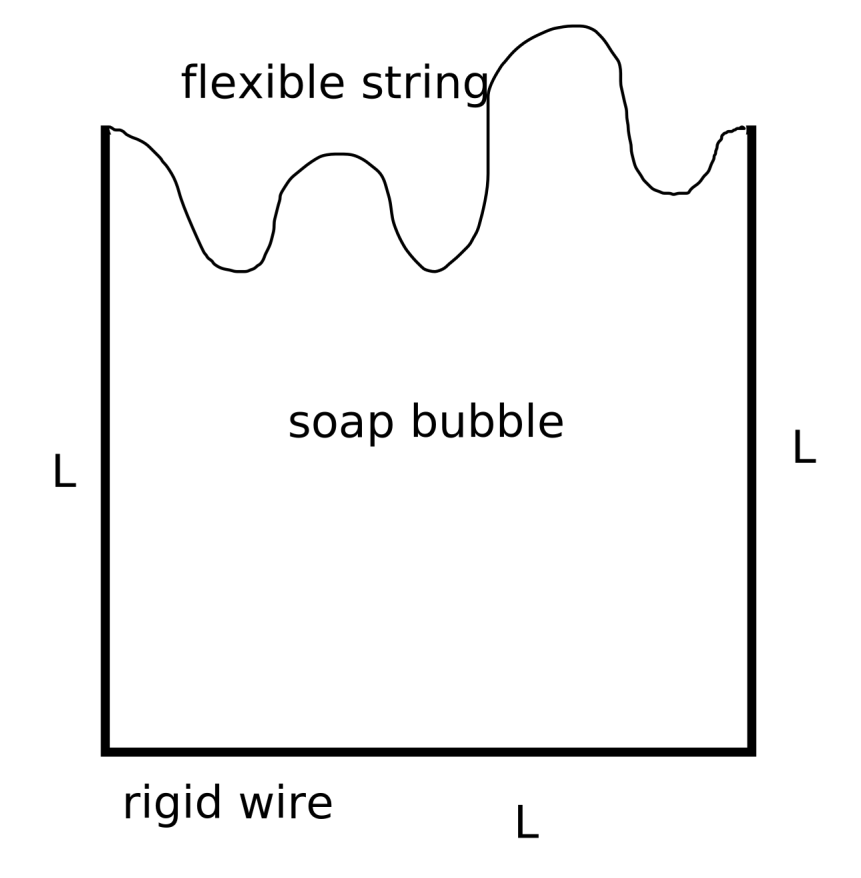
\includegraphics[width=4cm]{string-bubble.png}
\centering
\end{figure}

\begin{itemize}
    \item Write down an expression for the enclosed area using rectangular coordinates $x$ and $y$.
    \item Write down an expression for the relevant constraint.
    \item Use the Euler-Lagrange equation to minimize the enclosed area. 
    Show that the resulting differential equation is:
    $$
    \frac{dy}{dx} = \frac{ \sqrt{ \lambda^2 - \left( y - y_0 \right)^2 } }{y - y_0}
    \quad\quad\text{where $y_0$ and $\lambda$ are constants}
    $$
    Hint: when $f(y, y', x)$ doesn't include $x$, the EL equation can be written: 
    $$
    \frac{\partial f}{\partial y} - \frac{d}{dx} \frac{\partial f}{\partial y'} = 0
    \quad\quad\rightarrow\quad\quad
    f - y' \frac{\partial f}{\partial y'} = \text{constant}
    $$
    \item Separate and solve the differential equation. 
    
    Hint: Try the substitution $\sin u = \tfrac{y - y_0}{\lambda}$
    \item There is a common name for the resulting curve. What is it? (For example: catenary, circle, cosine, ellipse, hyperbola, parabola, etc)
    \item Draw a diagram of the solution. Based on that diagram, write down an equation to solve for each undetermined constant.
    \item Let $L=10\,\text{cm}$ and $\ell=20\,\text{cm}$. Solve numerically for the values of each undetermined constant. You may use Mathematica or Wolfram Alpha on this part.
    
\end{itemize}

\newpage
\section*{For Reference}

Taylor does not cover this usage of Lagrange multipliers. 

Suppose you have a quantity $A$ defined as:
$$
A = \displaystyle\int_{x_0}^{x_1} f(y, y', x) \; dx
\quad\quad\text{where $y' = \tfrac{dy}{dx}$}
$$
Suppose further that $y(x)$ is subject to a constraint of the form:
$$
\ell = \displaystyle\int_{x_0}^{x_1} g(y, y', x) \; dx
\quad\quad\text{where $\ell$ is fixed}
$$
You're looking for $y(x)$ that extremizes the value of $A$ while respecting the constraint. The solution is obtained by extremizing $A^*$:
$$
A^* = \displaystyle\int_{x_0}^{x_1} f(y, y', x) + \lambda \; g(y, y', x) \; dx
$$
Where $\lambda$ is an undetermined constant.

\newpage

We haven't used numerical solvers much. Here's a quick example:

\begin{figure}[h]
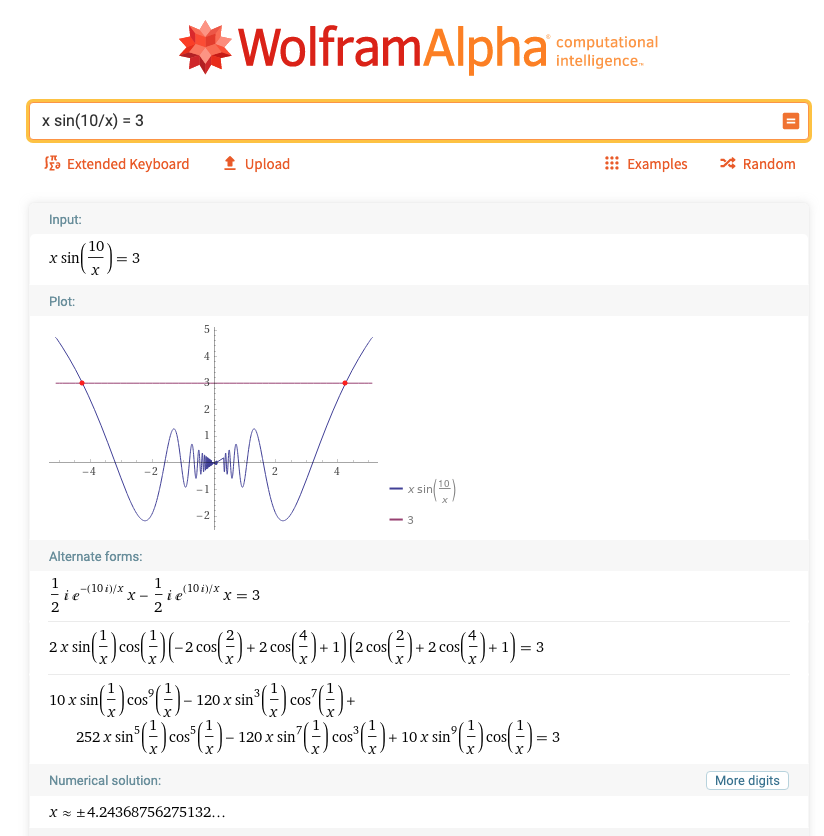
\includegraphics[width=12cm]{wolfram-solver-example.png}
\centering
\end{figure}


\end{document}
